\documentclass[12pt]{article}
\usepackage{times}
\usepackage[margin=1in]{geometry}
\usepackage{enumitem}
\setlist{nosep}
\usepackage{graphicx}
\usepackage{hyperref}
\usepackage{framed}
\usepackage{subcaption}
\usepackage{wrapfig}
\renewcommand{\rmdefault}{ptm} 
\usepackage{setspace}
\singlespacing
\usepackage{float}
\raggedbottom

\begin{document}


% Cover Page


\begin{titlepage}
    \begin{center}
        \begin{minipage}[c]{0.21\textwidth}
            
\includegraphics[width=\textwidth]{Cairo-University-CU-.png}
        \end{minipage}
        \hfill
        \begin{minipage}[c]{0.5\textwidth}
            \centering
            {\large Cairo University - Faculty Of Engineering \\EECE Department \\ Virtual Networks Lab using Linux and the CORE
            Network Emulator \par}
        \end{minipage}
        \hfill
        \begin{minipage}[c]{0.15\textwidth}
            
\includegraphics[width=\textwidth]{CUFE.png}
        \end{minipage}
    \end{center}
    \vspace*{2cm}
    \begin{center}
        \begin{tabular}{|c|c|c|}
            \hline
            \textbf{Name} & \textbf{Section} & \textbf{Bench Number} \\
            \hline
            Youssef Samir Zidan & 4 & 9220988 \\
            \hline
            Yassin Essam Yassin & 4 & 9220965 \\
            \hline
        \end{tabular}\\[2cm]
        \tableofcontents
    \end{center}
\end{titlepage}
\listoffigures

\vspace{-1em}
\section{Effect of TCP Window Size}
\subsection{Question 2.i}
The Throughout Appears to be increasing with Window Size (as Expected) with Zero Retransmissions up to a certain limit where the receiver Buffer gets Full at 6KB and tries to increase it's buffer size so performance is increases again thus making a zigzag type of graph, then at 24KB the Buffer can't get any larger so Performance is Poor.

$$Throughout=\frac{Data\:Transferred}{Interval\:Time}$$

\begin{figure}[!htbp]
    \centering
    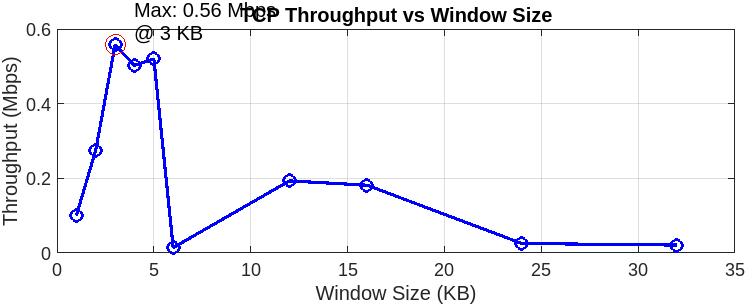
\includegraphics[width=0.9\textwidth]{Throughout_WS.png}
    \caption{TCP Window Size vs Throughput}
    \label{fig:throughput_ws}
\end{figure}
\begin{figure}[!htbp]
    \centering
    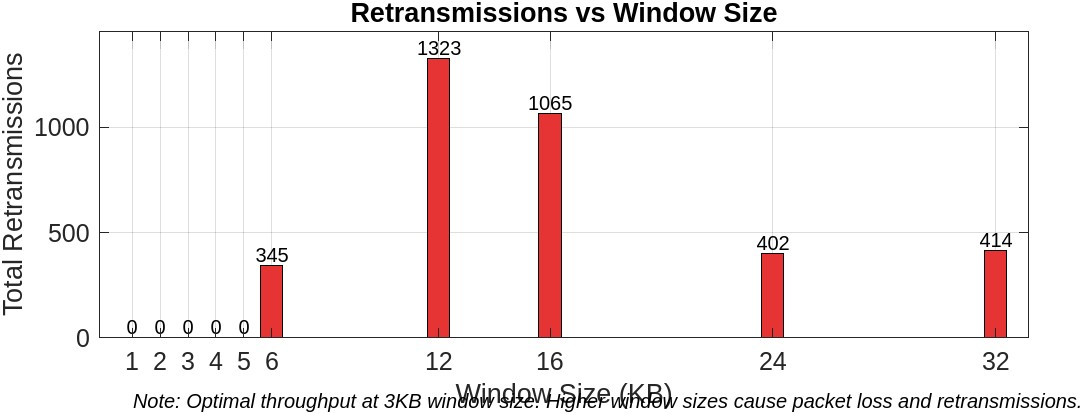
\includegraphics[width=0.9\textwidth]{Retransmissions_WS.jpg}
    \caption{TCP Window Size vs Retransmissions}
    \label{fig:retransmissions_ws}
\end{figure}

\begin{table}[!htbp]
    \centering
    \small
    \begin{tabular}{|c|c|c|c|}
        \hline
        \textbf{Window Size (KB)} & \textbf{Data (MB)} & \textbf{Throughput (MB/s)} & \textbf{Retransmissions} \\
        \hline
        1 & 4.01 & 0.10025 &0 \\
        2 & 11.00 & 0.27500 &0\\
        3 & 22.30 & 0.55750 &0\\
        4 & 20.10 & 0.50250 &0\\
        5 & 20.80 & 0.52000 &0\\
        6 & 0.58 & 0.01450 &345\\
        12 & 7.73 & 0.19325 &1323\\
        16 & 7.27 & 0.18175 &1065\\
        24 & 1.022 & 0.02555 &402\\
        32 & 0.853 & 0.021325 &404\\
        \hline
    \end{tabular}
    \caption{TCP Window Size vs Throughput Data}
    \label{tab:window_size_data}
\end{table}
\pagebreak
%\begin{framed}
%\footnotesize
%\noindent\textbf{Terminal Output:}
%\begin{verbatim}
%n7.conf# iperf3 -c 10.0.13.20 -t 40 -i 10 -w 1k
%Connecting to host 10.0.13.20, port 5201
%[4] local 10.0.12.20 port 60642 connected to 10.0.13.20 port 5201
%[ID] Interval           Transfer     Bandwidth       Retr  Cwnd
%[4]   0.00-10.00  sec  1.01 MBytes   845 Kbits/sec    0   5.45 KBytes       
%[4]  10.00-20.00  sec  1.00 MBytes   841 Kbits/sec    0   5.45 KBytes       
%[4]  20.00-30.00  sec  1.00 MBytes   840 Kbits/sec    0   5.45 KBytes       
%n7.conf# iperf3 -c 10.0.13.20 -t 40 -i 10 -w 1k
%Connecting to host 10.0.13.20, port 5201
%[4] local 10.0.12.20 port 60642 connected to 10.0.13.20 port 5201
%[ID] Interval           Transfer     Bandwidth       Retr  Cwnd
%[4]   0.00-10.00  sec  1.01 MBytes   845 Kbits/sec    0   5.45 KBytes       
%[4]  10.00-20.00  sec  1.00 MBytes   841 Kbits/sec    0   5.45 KBytes       
%[4]  20.00-30.00  sec  1.00 MBytes   840 Kbits/sec    0   5.45 KBytes       
%[4]  30.00-40.00  sec  1023 KBytes   838 Kbits/sec    0   5.45 KBytes       
%- - - - - - - - - - - - - - - - - - - - - - - - -
%[ ID] Interval           Transfer     Bandwidth       Retr
%[4]   0.00-40.00  sec  4.01 MBytes   841 Kbits/sec    0       sender
%[4]   0.00-40.00  sec  4.01 MBytes   841 Kbits/sec            receiver
%
%iperf Done.
%n7.conf# iperf3 -c 10.0.13.20 -t 40 -i 10 -w 2k
%Connecting to host 10.0.13.20, port 5201
%[4] local 10.0.12.20 port 60644 connected to 10.0.13.20 port 5201
%[ID] Interval           Transfer     Bandwidth       Retr  Cwnd
%[4]   0.00-10.00  sec  2.77 MBytes  2.32 Mbits/sec    0   7.07 KBytes       
%[4]  10.00-20.00  sec  2.71 MBytes  2.28 Mbits/sec    0   7.07 KBytes       
%[4]  20.00-30.00  sec  2.74 MBytes  2.30 Mbits/sec    0   7.07 KBytes       
%[4]  30.00-40.00  sec  2.78 MBytes  2.34 Mbits/sec    0   7.07 KBytes       
%- - - - - - - - - - - - - - - - - - - - - - - - -
%[ID] Interval           Transfer     Bandwidth       Retr
%[4]   0.00-40.00  sec  11.0 MBytes  2.31 Mbits/sec    0       sender
%[4]   0.00-40.00  sec  11.0 MBytes  2.31 Mbits/sec            receiver
%
%iperf Done.
%n7.conf# iperf3 -c 10.0.13.20 -t 40 -i 10 -w 3k
%Connecting to host 10.0.13.20, port 5201
%[4] local 10.0.12.20 port 60646 connected to 10.0.13.20 port 5201
%[ID] Interval           Transfer     Bandwidth       Retr  Cwnd
%[4]   0.00-10.00  sec  5.60 MBytes  4.70 Mbits/sec    0   14.1 KBytes       
%[4]  10.00-20.00  sec  5.57 MBytes  4.67 Mbits/sec    0   14.1 KBytes       
%[4]  20.00-30.00  sec  5.56 MBytes  4.66 Mbits/sec    0   14.1 KBytes       
%[4]  30.00-40.00  sec  5.55 MBytes  4.66 Mbits/sec    0   14.1 KBytes       
%- - - - - - - - - - - - - - - - - - - - - - - - -
%[ID] Interval           Transfer     Bandwidth       Retr
%[4]   0.00-40.00  sec  22.3 MBytes  4.67 Mbits/sec    0     sender
%[4]   0.00-40.00  sec  22.3 MBytes  4.67 Mbits/sec       receiver
%
%iperf Done.
%n7.conf# iperf3 -c 10.0.13.20 -t 40 -i 10 -w 4k
%Connecting to host 10.0.13.20, port 5201
%[4] local 10.0.12.20 port 60648 connected to 10.0.13.20 port 5201
%[ID] Interval           Transfer     Bandwidth       Retr  Cwnd
%[4]   0.00-10.00  sec  4.95 MBytes  4.15 Mbits/sec    0   14.1 KBytes       
%[4]  10.00-20.00  sec  5.01 MBytes  4.21 Mbits/sec    0   14.1 KBytes       
%[4]  20.00-30.00  sec  5.05 MBytes  4.24 Mbits/sec    0   14.1 KBytes       
%[4]  30.00-40.00  sec  5.10 MBytes  4.27 Mbits/sec    0   14.1 KBytes       
%- - - - - - - - - - - - - - - - - - - - - - - - -
%[ID] Interval           Transfer     Bandwidth       Retr
%[4]   0.00-40.00  sec  20.1 MBytes  4.22 Mbits/sec    0    sender
%[4]   0.00-40.00  sec  20.1 MBytes  4.22 Mbits/sec      receiver
%
%iperf Done.
%n7.conf# iperf3 -c 10.0.13.20 -t 40 -i 10 -w 5k
%Connecting to host 10.0.13.20, port 5201
%[4] local 10.0.12.20 port 60650 connected to 10.0.13.20 port 5201
%[ID] Interval           Transfer     Bandwidth       Retr  Cwnd
%[4]   0.00-10.00  sec  5.21 MBytes  4.37 Mbits/sec    0   14.1 KBytes       
%[4]  10.00-20.00  sec  5.20 MBytes  4.36 Mbits/sec    0   14.1 KBytes       
%[4]  20.00-30.00  sec  5.24 MBytes  4.40 Mbits/sec    0   14.1 KBytes       
%[4]  30.00-40.00  sec  5.16 MBytes  4.33 Mbits/sec    0   14.1 KBytes       
%- - - - - - - - - - - - - - - - - - - - - - - - -
%[ID] Interval           Transfer     Bandwidth       Retr
%[4]   0.00-40.00  sec  20.8 MBytes  4.36 Mbits/sec    0  sender
%[4]   0.00-40.00  sec  20.8 MBytes  4.36 Mbits/sec       receiver
%
%iperf Done.
%n7.conf# iperf3 -c 10.0.13.20 -t 40 -i 10 -w 6k
%Connecting to host 10.0.13.20, port 5201
%[4] local 10.0.12.20 port 60652 connected to 10.0.13.20 port 5201
%[ID] Interval           Transfer     Bandwidth       Retr  Cwnd
%[4]   0.00-10.00  sec   154 KBytes   126 Kbits/sec   86   4.24 KBytes       
%[4]  10.00-20.00  sec   139 KBytes   114 Kbits/sec   85   4.24 KBytes       
%[4]  20.00-30.00  sec   143 KBytes   117 Kbits/sec   87   4.24 KBytes       
%[4]  30.00-40.00  sec   144 KBytes   118 Kbits/sec   87   4.24 KBytes       
%- - - - - - - - - - - - - - - - - - - - - - - - -
%[ ID] Interval           Transfer     Bandwidth       Retr
%[4]   0.00-40.00  sec   580 KBytes   119 Kbits/sec  345     sender
%[4]   0.00-40.00  sec   570 KBytes   117 Kbits/sec          receiver
%
%iperf Done.
%n7.conf# iperf3 -c 10.0.13.20 -t 40 -i 10 -w 12k
%Connecting to host 10.0.13.20, port 5201
%[4] local 10.0.12.20 port 60654 connected to 10.0.13.20 port 5201
%[ID] Interval           Transfer     Bandwidth       Retr  Cwnd
%[4]   0.00-10.00  sec  1.74 MBytes  1.46 Mbits/sec  286   2.83 KBytes       
%[4]  10.00-20.00  sec  1.76 MBytes  1.48 Mbits/sec  283   4.24 KBytes       
%[4]  20.00-30.00  sec  2.05 MBytes  1.72 Mbits/sec  359   2.83 KBytes       
%[4]  30.00-40.00  sec  2.18 MBytes  1.83 Mbits/sec  395   2.83 KBytes       
%- - - - - - - - - - - - - - - - - - - - - - - - -
%[ID] Interval           Transfer     Bandwidth       Retr
%[4]   0.00-40.00  sec  7.73 MBytes  1.62 Mbits/sec  1323  sender
%[4]   0.00-40.00  sec  7.72 MBytes  1.62 Mbits/sec        receiver
%
%iperf Done.
%n7.conf# iperf3 -c 10.0.13.20 -t 40 -i 10 -w 16k
%Connecting to host 10.0.13.20, port 5201
%[4] local 10.0.12.20 port 60656 connected to 10.0.13.20 port 5201
%[ID] Interval           Transfer     Bandwidth       Retr  Cwnd
%[4]   0.00-10.00  sec  1.77 MBytes  1.48 Mbits/sec  268   4.24 KBytes       
%[4]  10.00-20.00  sec  1.85 MBytes  1.55 Mbits/sec  268   4.24 KBytes       
%[4]  20.00-30.00  sec  1.85 MBytes  1.55 Mbits/sec  268   4.24 KBytes       
%[4]  30.00-40.00  sec  1.80 MBytes  1.51 Mbits/sec  261   4.24 KBytes       
%- - - - - - - - - - - - - - - - - - - - - - - - -
%[ID] Interval           Transfer     Bandwidth       Retr
%[4]   0.00-40.00  sec  7.27 MBytes  1.52 Mbits/sec  1065   sender
%[4]   0.00-40.00  sec  7.25 MBytes  1.52 Mbits/sec         receiver
%
%iperf Done.
%n7.conf# iperf3 -c 10.0.13.20 -t 40 -i 10 -w 24k
%Connecting to host 10.0.13.20, port 5201
%[4] local 10.0.12.20 port 60658 connected to 10.0.13.20 port 5201
%[ID] Interval           Transfer     Bandwidth       Retr  Cwnd
%[4]   0.00-10.00  sec   270 KBytes   221 Kbits/sec   97   5.66 KBytes       
%[4]  10.00-20.00  sec   218 KBytes   178 Kbits/sec   88   5.66 KBytes       
%[4]  20.00-30.00  sec   257 KBytes   211 Kbits/sec  106   8.48 KBytes       
%[4]  30.00-40.00  sec   277 KBytes   227 Kbits/sec  111   7.07 KBytes       
%- - - - - - - - - - - - - - - - - - - - - - - - -
%[ID] Interval           Transfer     Bandwidth       Retr
%[4]   0.00-40.00  sec  1022 KBytes   209 Kbits/sec  402   sender
%[4]   0.00-40.00  sec   981 KBytes   201 Kbits/sec        receiver
%
%iperf Done.
%n7.conf# iperf3 -c 10.0.13.20 -t 40 -i 10 -w 32k
%Connecting to host 10.0.13.20, port 5201
%[4] local 10.0.12.20 port 60660 connected to 10.0.13.20 port 5201
%[ID] Interval           Transfer     Bandwidth       Retr  Cwnd
%[4]   0.00-10.00  sec   288 KBytes   236 Kbits/sec  109   9.90 KBytes       
%[4]  10.00-20.00  sec   161 KBytes   132 Kbits/sec   94   21.2 KBytes       
%[4]  20.00-30.00  sec   214 KBytes   175 Kbits/sec  113   7.07 KBytes       
%[4]  30.00-40.00  sec   189 KBytes   155 Kbits/sec   98   15.6 KBytes       
%- - - - - - - - - - - - - - - - - - - - - - - - -
%[ID] Interval           Transfer     Bandwidth       Retr
%[4]   0.00-40.00  sec   853 KBytes   175 Kbits/sec  414    sender
%[4]   0.00-40.00  sec   803 KBytes   164 Kbits/sec         receiver
%    \end{verbatim}
%\end{framed}

\subsection{Question 2.ii}
Frame length is 76 bytes \newline
IPv4 Header length : 20 bytes \newline
TCP header length : 40 bytes\newline
Ethernet = 16 bytes

\begin{figure}[!htbp]
    \centering
    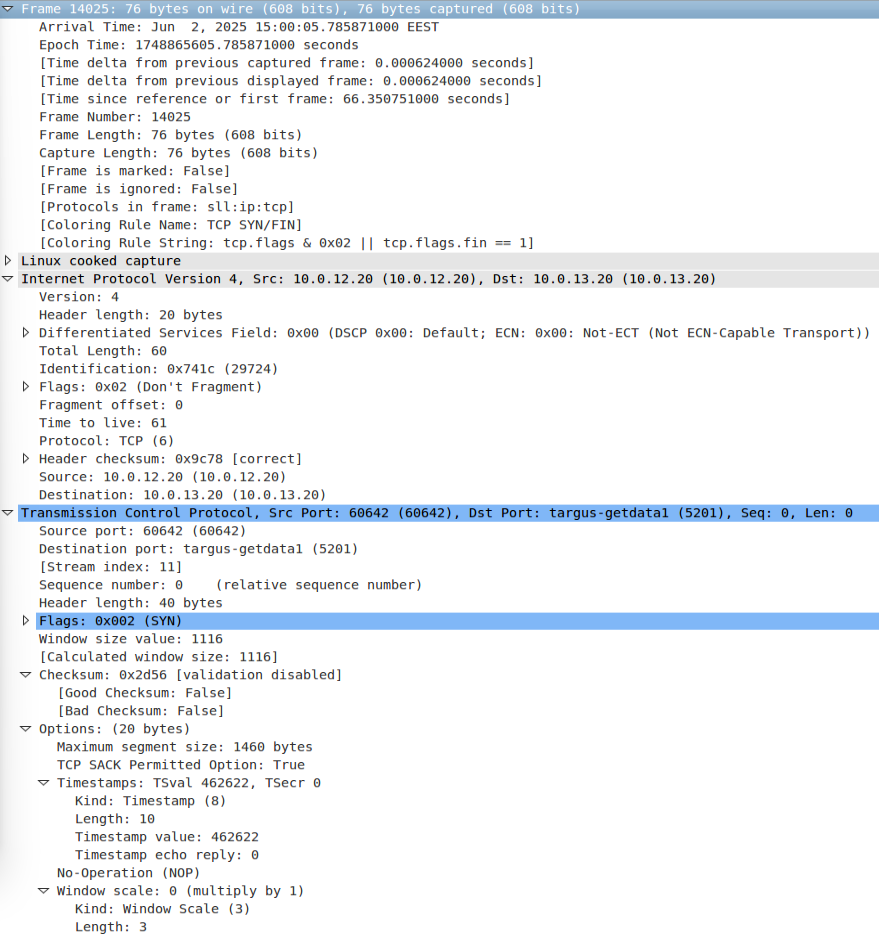
\includegraphics[width=0.95\textwidth]{packet_sent.png}
    \caption{Sent packet from node n7}
    \label{fig:Sent_packet}
\end{figure}
\pagebreak
\subsection{Question 2.iii}
Frame length is 68 bytes \newline
IPv4 Header length : 20 bytes \newline
TCP header length : 32 bytes\newline
Ethernet = 16 bytes \newline
Ack number = 42 \& Sequance No. = 2 (Both Relative)
\begin{figure}[!htbp]
    \centering
    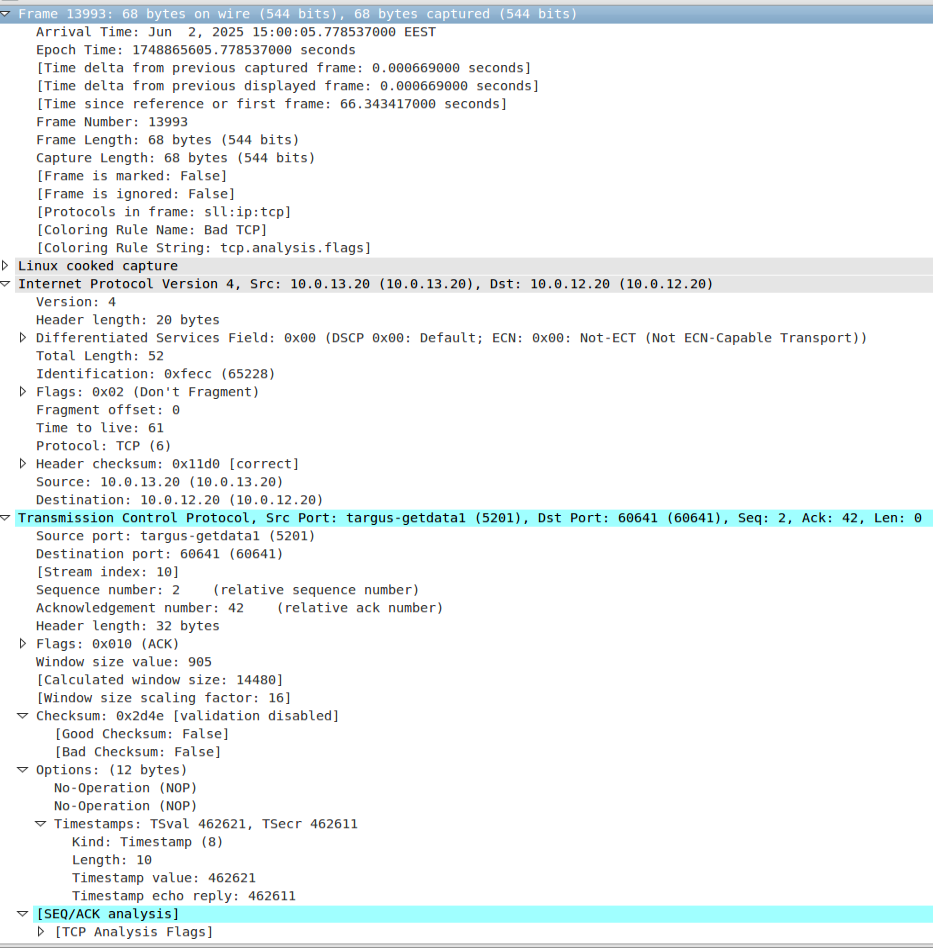
\includegraphics[width=0.95\textwidth]{ack_rec.png}
    \caption{Received from node n11}
    \label{fig:Received_packet}
\end{figure}
\section{TCP Short versus Long Paths}
\subsection{Question 3.i}
The Lower Performance is due to larger Delay between n7 \& n8 ($4*160+2*110\mu$sec) compared to n7 \& n11($3*160+110\mu$sec)
\begin{framed}
    \footnotesize
    \noindent\textbf{Terminal Output:}
    \begin{verbatim}
64 bytes from 10.0.11.20: icmp_req=3 ttl=59 time=6.04 ms
^Z
[1]+  Stopped                 ping 10.0.11.20
n7.conf# iperf3 -c 10.0.11.20 -t 40 -i 10 -w 4k
Connecting to host 10.0.11.20, port 5201
[4] local 10.0.12.20 port 48635 connected to 10.0.11.20 port 5201
[ID] Interval           Transfer     Bandwidth       Retr  Cwnd
[4]   0.00-10.00  sec  2.00 MBytes  1.68 Mbits/sec    1   8.48 KBytes       
[4]  10.00-20.00  sec  1.71 MBytes  1.44 Mbits/sec    0   8.48 KBytes       
[4]  20.00-30.12  sec  1.63 MBytes  1.35 Mbits/sec    0   8.48 KBytes       
[4]  30.12-40.00  sec  1.94 MBytes  1.64 Mbits/sec    4   8.48 KBytes       
- - - - - - - - - - - - - - - - - - - - - - - - -
[ID] Interval           Transfer     Bandwidth       Retr
[4]   0.00-40.00  sec  7.28 MBytes  1.53 Mbits/sec    5             sender
[4]   0.00-40.00  sec  7.27 MBytes  1.53 Mbits/sec                  receiver
iperf Done.
\end{verbatim}
\end{framed}
\begin{table}[H]
    \centering
    \begin{tabular}{|c|c|c|}
        \hline
        \textbf{Window Size (KB)} & \textbf{Data (MB)} & \textbf{Throughput (MB/s)} \\
        \hline

        4(old) & 20.10 & 0.50250 \\
        4(new) & 7.28 & 0.182 \\
        \hline
    \end{tabular}
    \caption{TCP With Different Propagation Delay}
    \label{tab:window_size_data}
\end{table}
\pagebreak
\section{Higher Link Capacity with Drops versus Reliable Lower Capacity}
\begin{table}[!htbp]
    \centering
    \small
    \begin{tabular}{|c|c|c|c|c|}
        \hline
        \textbf{Case \#} & \textbf{Data (MB)} & \textbf{Throughput (MB/s)} & \textbf{Throughput (Mbps)} & \textbf{Retransmissions} \\
        \hline
        A & 10.10 & 0.2525 & 2.13 & 4 \\
        B & 9.91 & 0.2478 & 2.08 & 2 \\
        C & 2.09 & 0.0523 & 0.438 & 108 \\
        D & 0.728 & 0.0182 & 0.149 & 91 \\
        E & 6.70 & 0.1675 & 1.41 & 56 \\
        F & 8.74 & 0.2185 & 1.83 & 25 \\
        \hline
    \end{tabular}
    \caption{4KB Window Size Performance Variability (40-second tests)}
    \label{tab:4kb_window_tests}
\end{table}
\subsection{Question 4.i}
Throughout in case A is the best among these results due to high rate and no loss (Highest Capacity)

Also Case B is better Than C as the Bandwidth isn't really an issue with this window Size So Loss from both directions Really Impacts the Performance of Retransmissions and thus the throughput
\subsection{Question 4.ii}
Case B is better as there's no loss with adequate Capacity For given window Size unlike C which ReTransmits packets 
\subsection{Question 4.iii}
Case E is better Loss in the direction from n4 to n5 is Just Dropped Acks which doesn't effect the throughput that much especially in Go-BACK-N protocol

\section{OSPF Link Cost Changes}
\begin{figure}[H]
    \centering
    \begin{minipage}{0.75\textwidth}
        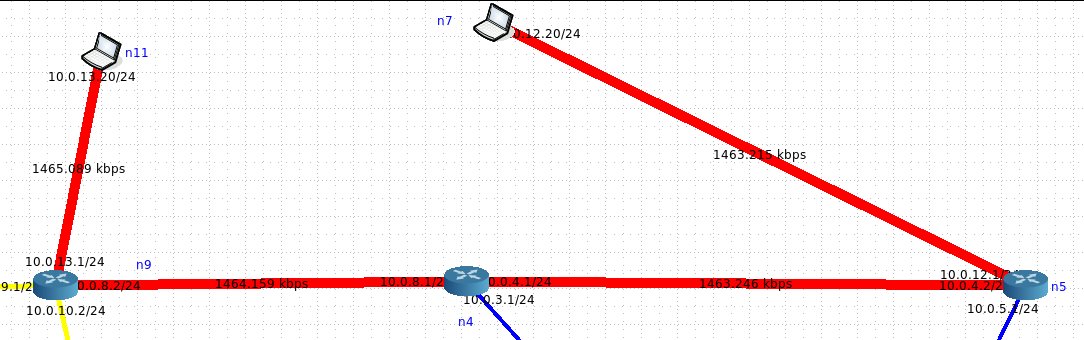
\includegraphics[width=\textwidth]{new_Sss/5.3 path.png}
    \end{minipage}%
    \begin{minipage}{0.2\textwidth}
        \caption{Path between n7 and n11}
        \label{fig:5.3-path}
    \end{minipage}
\end{figure}
\subsection{Question 5.i}
in Figure \ref{fig:5.i-a}, when the cost was changed to 40,the path changed from node 4 to node 6 as in Figure:\ref{fig:5i-NewPath} the traceroute changed  (in graph \ref{fig:5.i-b}),also the Throughput Slightly decreased ,Which's due to Cost.
\begin{figure}[H]
    \centering
    \begin{subfigure}[b]{0.48\textwidth}
        \centering
        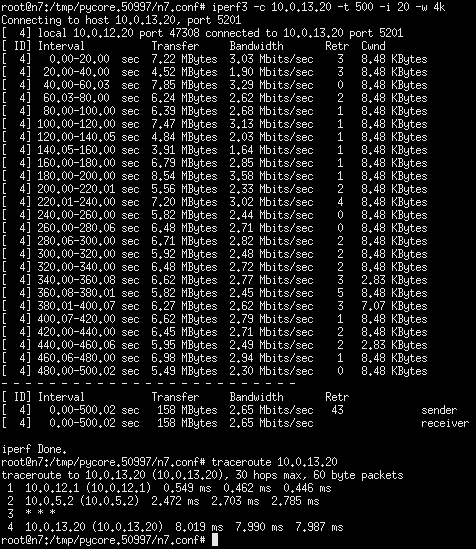
\includegraphics[width=\textwidth]{new_Sss/5.i cost 40.png}
        \caption{Cost Changed to 40}
        \label{fig:5.i-a}
    \end{subfigure}
    \hfill
    \begin{subfigure}[b]{0.48\textwidth}
        \centering
        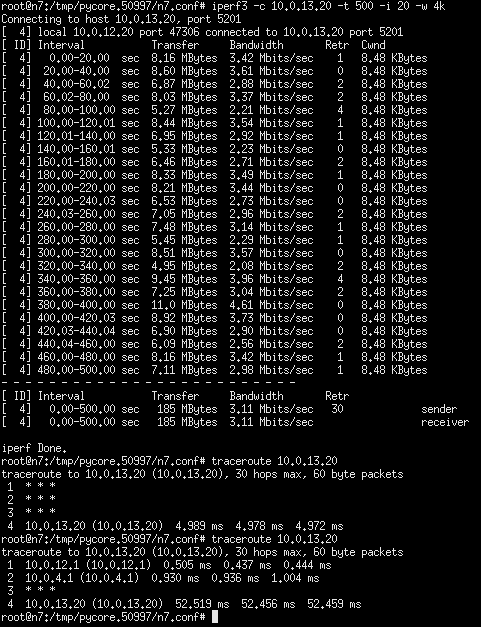
\includegraphics[width=\textwidth]{new_Sss/5.i cost 10.png}
        \caption{Before Changing The Cost}
        \label{fig:5.i-b}
    \end{subfigure}
    \caption{Network performance analysis}
    \label{fig:5.i}
\end{figure}


\begin{figure}[H]
    \centering
    \begin{minipage}{0.6\textwidth}
        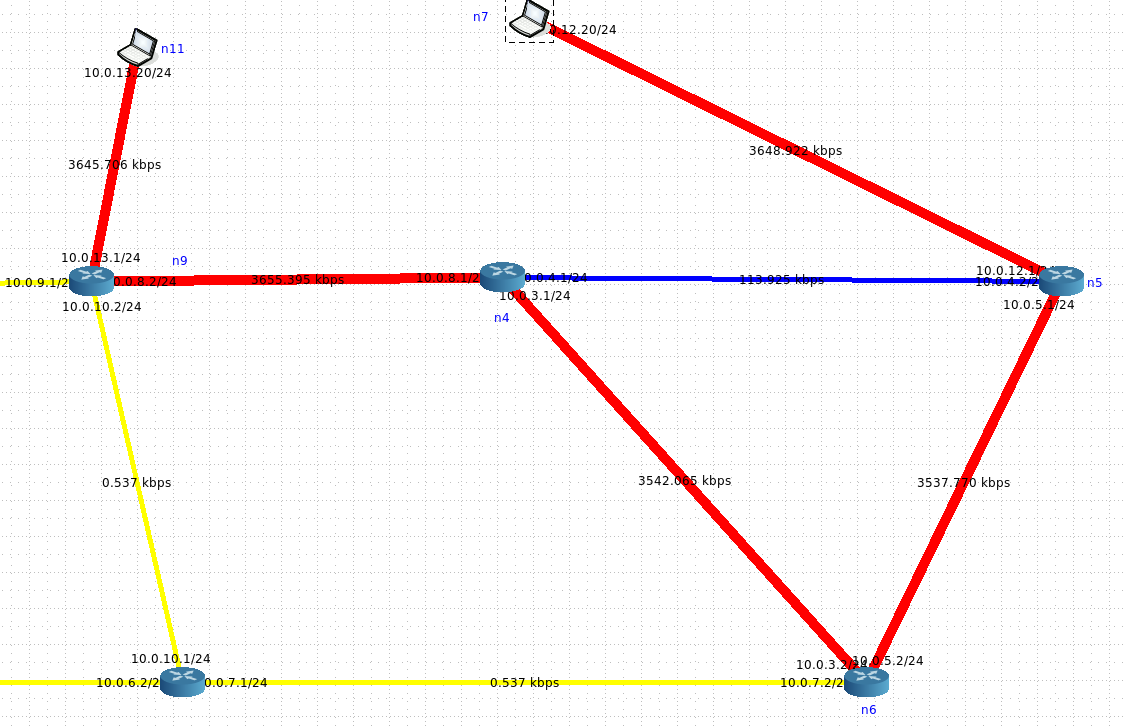
\includegraphics[width=\textwidth]{new_Sss/5.i new path.png}
    \end{minipage}%
    \begin{minipage}{0.3\textwidth}
        \captionof{figure}{New path after cost change}
        \label{fig:5i-NewPath}
    \end{minipage}
\end{figure}
\pagebreak
\subsection{Question 5.ii}
as the cost change from node 4 to node 5 the transfer from node 11 to node 7 decreased Slightly and the bandwidth by changing it's route, while for node 7 to node 11 it doesn't get effected as the cost from node 5 to 4 is 10

\begin{figure}[H]
    \centering
    \begin{subfigure}[b]{0.75\textwidth}
        \centering
        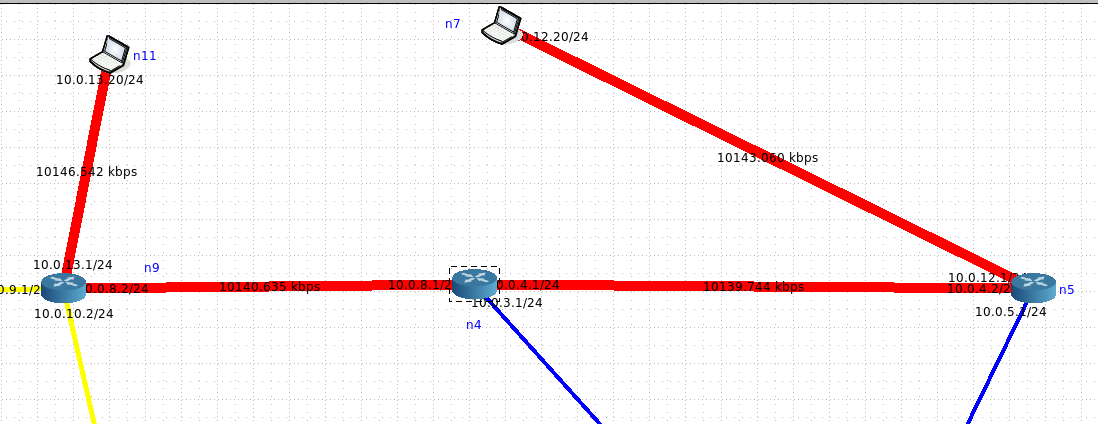
\includegraphics[width=\textwidth]{new_Sss/5.ii old path.png}
        \caption{Original Path}
        \label{fig:5ii-OldPath}
    \end{subfigure}
    
    \vspace{0.5em}
    
    \begin{subfigure}[b]{0.75\textwidth}
        \centering
        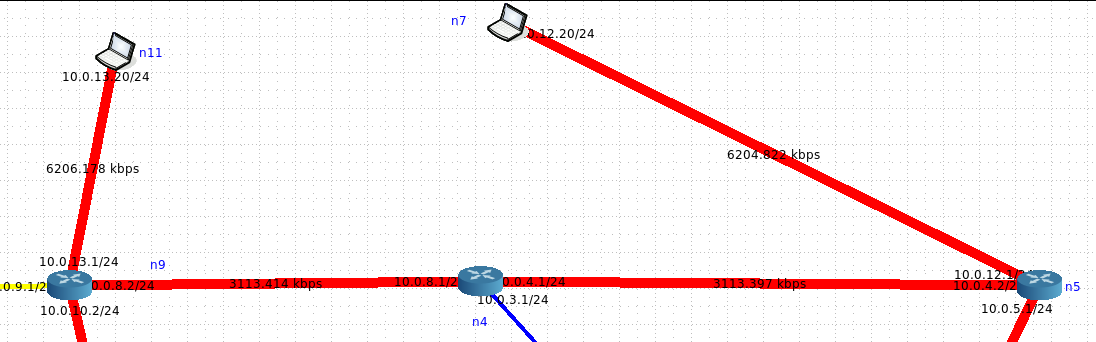
\includegraphics[width=\textwidth]{new_Sss/5.ii n7 new path.png}
        \caption{New Path N7}
        \label{fig:5ii-Path1}
    \end{subfigure}
    
    \vspace{0.5em}
    
    \begin{subfigure}[b]{0.75\textwidth}
        \centering
        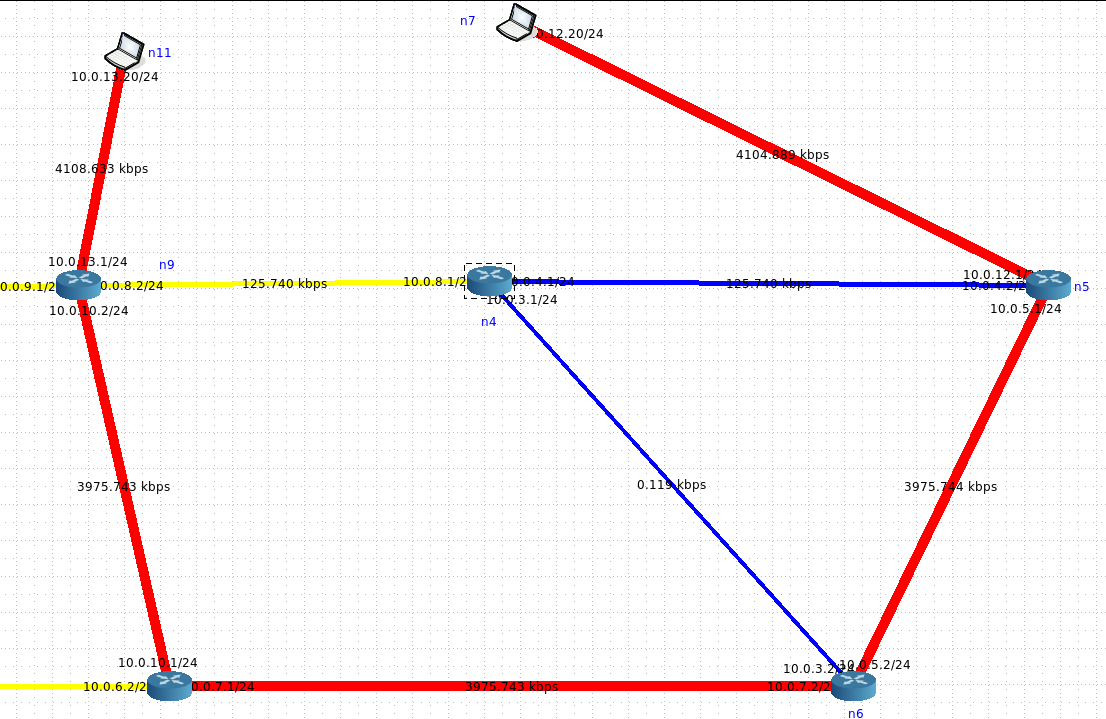
\includegraphics[width=\textwidth]{new_Sss/5.ii n11 new path.png}
        \caption{New Path N11}
        \label{fig:5ii-Path2}
    \end{subfigure}
    \caption{Network paths before and after cost changes}
    \label{fig:5ii-paths}
\end{figure}

\begin{figure}[H]
    \centering
    \begin{subfigure}{0.45\textwidth}
        \centering
        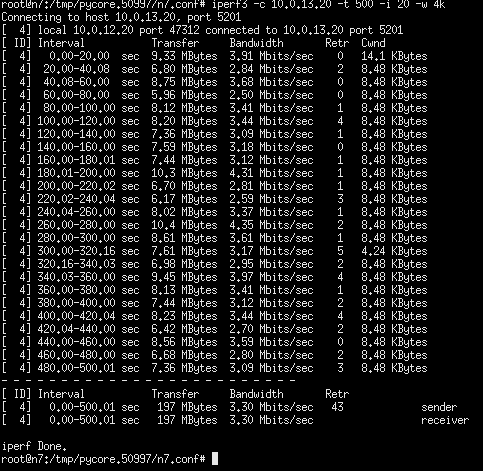
\includegraphics[width=1\textwidth]{new_Sss/5.ii n7 cost 10.png}
        \caption{Node 7 to Node 11 (cost=10)}
        \label{fig:5ii-a}
    \end{subfigure}
    \hspace{1.3em}
    \begin{subfigure}{0.45\textwidth}
        \centering
        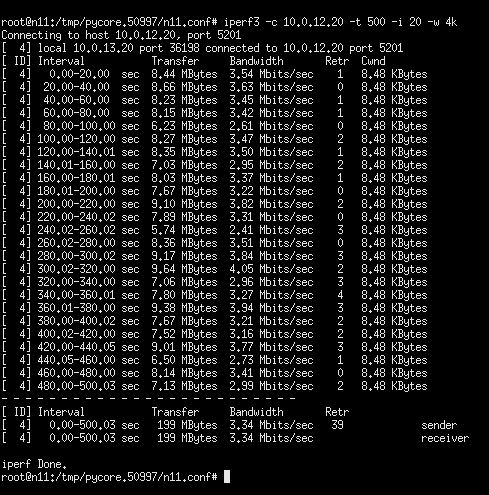
\includegraphics[width=1\textwidth]{new_Sss/5.ii n11 cost 10.png}
        \caption{Node 11 to Node 7 (cost=10)}
        \label{fig:5ii-b}
    \end{subfigure}

    \vspace{0.5em}

    \begin{subfigure}{0.45\textwidth}
        \centering
        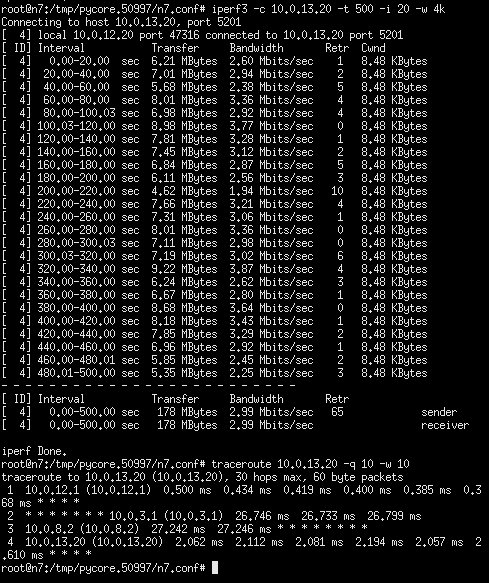
\includegraphics[width=1\textwidth]{new_Sss/5.ii n7 cost 40.png}
        \caption{Node 7 to Node 11 (cost=40)}
        \label{fig:5ii-c}
    \end{subfigure}
    \hspace{1.3em}
    \begin{subfigure}{0.45\textwidth}
        \centering
        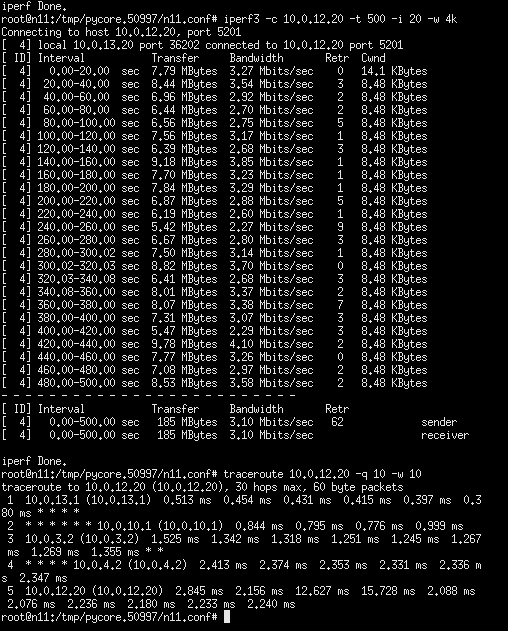
\includegraphics[width=1\textwidth]{new_Sss/5.ii n11 cost 40.png}
        \caption{Node 11 to Node 7 (cost=40)}
        \label{fig:5ii-d}
    \end{subfigure}

    \caption{Network performance before and after changing the interface cost}
    \label{fig:5.ii}
\end{figure}

\vspace{-1em}


\pagebreak
\section{OSPF Database Updates}
%\subsection*{Setup}
%\begin{enumerate}
%    \item Start wireshark and have its filter to capture only OSPF related packets.
%    \item Go to router n2, open vtysh and issue the commands:
%    \begin{verbatim}
%    config terminal
%    show ip ospf database
%    show ip ospf route
%    \end{verbatim}
%    \item On router n4, set link cost of eth1 to 20. Capture the link state packets advertised in wireshark.
%    \item Go to router n4, go out of vtysh, or open new bash terminal and issue the following commands:
%    \begin{verbatim}
%    ifconfig eth0 down
%    ifconfig eth1 down
%    ifconfig eth2 down
%    \end{verbatim}
%\end{enumerate}

\subsection{Question 6.i}
\begin{figure}[H]
    \hfill
    \begin{minipage}{0.95\textwidth}
        \begin{minipage}{0.4\textwidth}
            as destination have the same cost and ospf support equal cost multiplath so there are more than path has the same cost. So, switch can select any one of them. Also, if one of the paths is down, there should be another one.
        \end{minipage}
        \hfill
        \begin{minipage}{0.5\textwidth}
            \centering
            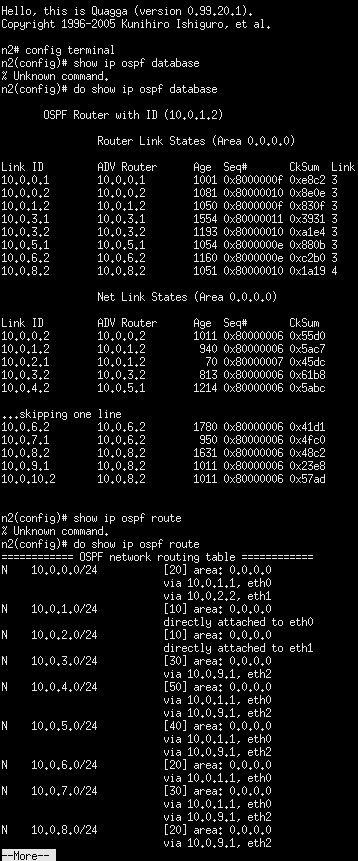
\includegraphics[width=\textwidth]{new_Ss/6.i.png}
            \caption{OSPF Routing Table Router n2}
            \label{fig:6.i}
        \end{minipage}
    \end{minipage}
\end{figure}
\pagebreak
\subsection{Question 6.ii}


    \begin{figure}[H]
        \centering
        \begin{subfigure}[b]{0.85\textwidth}
            \centering
            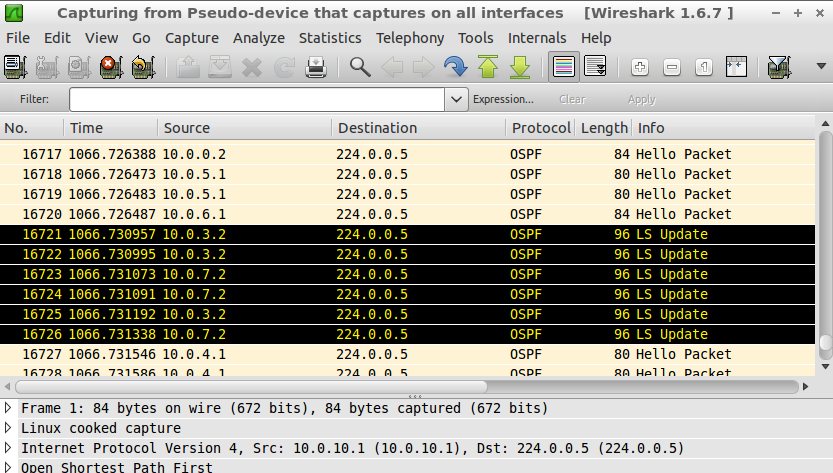
\includegraphics[width=\textwidth]{new_Ss/6.ii.1.png}
            \caption{First OSPF Update Message}
        \end{subfigure}
        \vskip\baselineskip
        \begin{subfigure}[b]{0.85\textwidth}
            \centering
            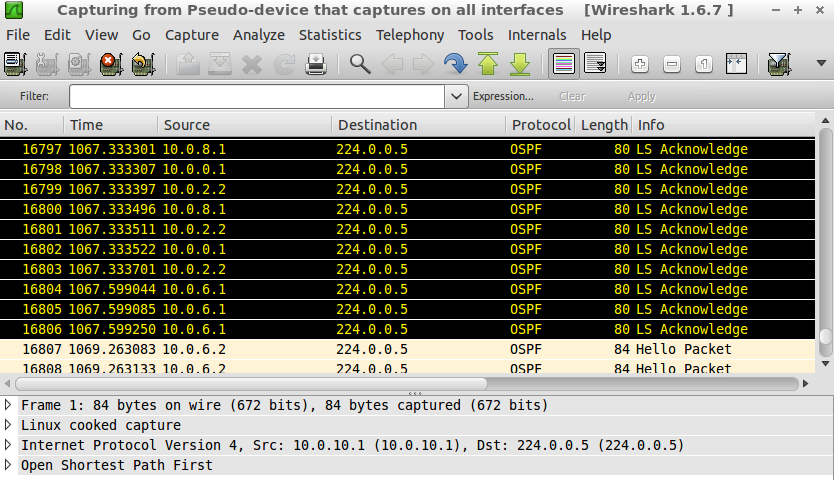
\includegraphics[width=\textwidth]{new_Ss/6.ii.2.png}
            \caption{Last ACK Message}
        \end{subfigure}
        \caption{OSPF Link State Exchange Timing Analysis}
        \label{fig:6.ii}
    \end{figure}

    $$time = t1 - t2 = 1,\!067.599250 - 1,\!066.730957 = 0.868293 sec$$

\subsection{Question 6.iii}

\begin{figure}[H]
    \hfill
    \begin{minipage}{1\textwidth}
        \begin{minipage}{0.3\textwidth}
            When we disconnect the N4 node, there should be another node to take its place
        \end{minipage}
        \hfill
        \begin{minipage}{0.5\textwidth}
            \centering
            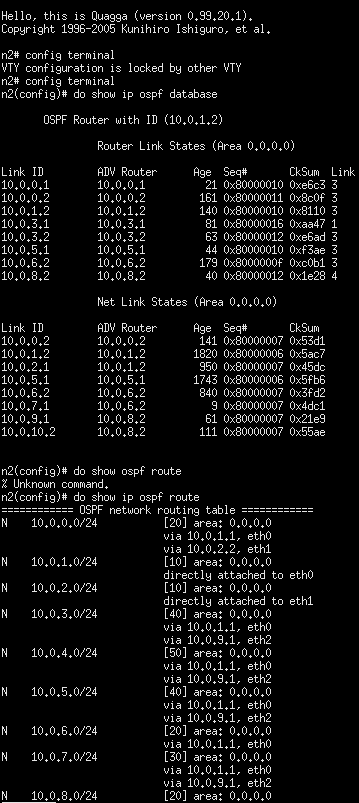
\includegraphics[width=\textwidth]{new_Ss/6.iii.png}
            \caption{New Routing Table}
            \label{fig:6.iii}
        \end{minipage}
    \end{minipage}
\end{figure}
\end{document} 